\documentclass[10pt,spanish]{article}  
\usepackage[spanish]{babel} %Indica que escribiermos en español
\usepackage[utf8]{inputenc} %Indica qué codificación se está usando ISO-8859-1(latin1)  o utf8 
\selectlanguage{spanish}

%%%%%%% DEFINICIÓN DE VARIABLES %%%%%%%%%%%%%%%%%%%
\newcommand{\Tarea}{Tarea \{ \# \}}
\newcommand{\Titulo}{Informe del Modelo de Diseño}
\newcommand{\Materia}{\{ MATERIA \}}
\newcommand{\Curso}{Curso \{ AÑO \}}
\newcommand{\Grupo}{Grupo \{ NRO \}}
% Nombre y Cedulas de los integrantes del grupo
\newcommand{\NomIntegrUno}{Integrante 1}
\newcommand{\CiIntegrUno}{CI}
\newcommand{\NomIntegrDos}{Integrante 2}
\newcommand{\CiIntegrDos}{CI}
\newcommand{\NomIntegrTres}{Integrante 3}
\newcommand{\CiIntegrTres}{CI}
\newcommand{\NomIntegrCuatro}{Integrante 4}
\newcommand{\CiIntegrCuatro}{CI}
\newcommand{\NomIntegrCinco}{Integrante 5}
\newcommand{\CiIntegrCinco}{CI}
% Nombre del Docente
\newcommand{\NomDocente}{Nombre Docente}
% Texto del Encabezado
\newcommand{\EncabezadoIzq}{Universidad de la República}
\newcommand{\EncabezadoMed}{Facultad de Ingeniería}
\newcommand{\EncabezadoDer}{Instituto de Computación}

%%%%%%%% PREÁMBULO %%%%%%%%%%%%

\usepackage{amsmath} % Comandos extras para matemáticas (cajas para ecuaciones,
% etc)
\usepackage{amssymb} % Simbolos matematicos (por lo tanto)

\usepackage{graphicx} % Incluir imágenes en LaTeX
\usepackage{color} % Para colorear texto
\usepackage{subfigure} % subfiguras
\usepackage{float} %Podemos usar el especificador [H] en las figuras para que se queden donde queramos
\usepackage{capt-of} % Permite usar etiquetas fuera de elementos flotantes
% (etiquetas de figuras)
\usepackage{sidecap} % Para poner el texto de las imágenes al lado
	\sidecaptionvpos{figure}{c} % Para que el texto se alinie al centro vertical
\usepackage{caption} % Para poder quitar numeracion de figuras
\usepackage{commath} % funcionalidades extras para diferenciales, integrales,
% etc (\od, \dif, etc)
\usepackage{cancel} % para cancelar expresiones (\cancelto{0}{x})
\usepackage{tabularx}

% MARGENES 
\usepackage{anysize} 					% Para personalizar el ancho de  los márgenes
\marginsize{2cm}{2cm}{2cm}{2cm} % Izquierda, derecha, arriba, abajo
\setlength{\parindent}{0cm}
\setlength{\parskip}{\baselineskip}

% Para que las referencias sean hipervínculos a las figuras o ecuaciones aparezcan en color
\usepackage[colorlinks=true,plainpages=true,citecolor=blue,linkcolor=blue]{hyperref}
%\usepackage{hyperref} 

% ENCABEZADO Y PIE DE PÁGINA
\usepackage{fancyhdr} 
\pagestyle{fancy}
\fancyhf{}

\fancyhead[L]{\EncabezadoIzq} %encabezado izquierda
\fancyhead[C]{\EncabezadoMed} %encabezado centro
\fancyhead[R]{\EncabezadoDer}   % dereecha

\fancyfoot[R]{\Curso}  % Pie derecha
\fancyfoot[C]{\thepage}  % centro
\fancyfoot[L]{\Tarea}  %izquierda
\renewcommand{\footrulewidth}{0.4pt}

\usepackage[framemethod=tikz]{mdframed}
\newmdenv[
  topline=false, %oculta linea arriba
  bottomline=false, % oculta linea abajo
  rightline=false, % oculta linea derecha
  skipabove=\topsep,
  skipbelow=\topsep,
]{siderules}

\numberwithin{figure}{section} % numeración de figuras por seccion
\usepackage[font=bf,labelfont=bf]{caption} % setea estilo bf (bold) a los caption (texto y label)

\usepackage[compact]{titlesec} %Formato de las secciones
\titleformat*{\section}{\LARGE\bfseries}
\titleformat*{\subsection}{\Large\bfseries}
\titleformat*{\subsubsection}{\large\bfseries}
\titlespacing{\section}{0pt}{-1ex}{-1.5ex}
\titlespacing{\subsection}{0pt}{-1ex}{-1.5ex}
\titlespacing{\subsubsection}{0pt}{-1ex}{-1.5ex}



\usepackage{etoolbox} % Agrega puntos a las sections en el TOC
\makeatletter
\patchcmd{\l@section}
  {\hfil}
  {\leaders\hbox{\normalfont$\m@th\mkern \@dotsep mu\hbox{.}\mkern \@dotsep mu$}\hfill}
  {}{}
\makeatother

% Corrige los margenes en las tablas
\setlength{\tabcolsep}{.5em}

% 4to nivel de subsections
\usepackage{hyperref}

\titleclass{\subsubsubsection}{straight}[\subsection]

\newcounter{subsubsubsection}[subsubsection]
\renewcommand\thesubsubsubsection{\thesubsubsection.\arabic{subsubsubsection}}
\renewcommand\theparagraph{\thesubsubsubsection.\arabic{paragraph}} % optional; useful if paragraphs are to be numbered

\titleformat{\subsubsubsection}
  {\normalfont\normalsize\bfseries}{\thesubsubsubsection}{1em}{}
\titlespacing*{\subsubsubsection}
{0pt}{3.25ex plus 1ex minus .2ex}{1.5ex plus .2ex}

\makeatletter
\renewcommand\paragraph{\@startsection{paragraph}{5}{\z@}%
  {3.25ex \@plus1ex \@minus.2ex}%
  {-1em}%
  {\normalfont\normalsize\bfseries}}
\renewcommand\subparagraph{\@startsection{subparagraph}{6}{\parindent}%
  {3.25ex \@plus1ex \@minus .2ex}%
  {-1em}%
  {\normalfont\normalsize\bfseries}}
\def\toclevel@subsubsubsection{4}
\def\toclevel@paragraph{5}
\def\toclevel@paragraph{6}
\def\l@subsubsubsection{\@dottedtocline{4}{7em}{4em}}
\def\l@paragraph{\@dottedtocline{5}{10em}{5em}}
\def\l@subparagraph{\@dottedtocline{6}{14em}{6em}}
\makeatother

\setcounter{secnumdepth}{4}
\setcounter{tocdepth}{4}

%easylist
\usepackage{easylist}

\title{\Tarea - \Titulo}

%%%%%%%% TERMINA PREÁMBULO %%%%%%%%%%%%

\begin{document}

%%%%%%%%%%%%%%%%%%%%%%%%%%%%%%%%%% PORTADA %%%%%%%%%%%%%%%%%%%%%%%%%%%%%%%%%%%%%%%%%%%%
\begin{minipage}{0.48\textwidth} \begin{flushleft}
\end{flushleft}\end{minipage}

%%%
\begin{center}																		%%%
\newcommand{\HRule}{\rule{\linewidth}{0.5mm}}									%%%\left
 																					%%%


													 								%%%
\vspace*{1cm}								%%%
																				%%%	
\textsc{\huge \Materia}\\[1.5cm]	

\textsc{\huge \Tarea				%%%
}\\[1.5cm]													%%%

    																				%%%
\vspace*{1cm}																		%%%
																					%%%
\HRule \\[0.4cm]																	%%%
{ \huge \bfseries \Titulo}\\[0.3cm]	%%%
 																					%%%
\HRule \\[4cm]																	%%%
 																				%%%
																					%%%
\begin{minipage}{0.8\textwidth}													%%%
\begin{flushleft} \large															%%%
\textsc{\LARGE \Grupo}\\
\LARGE{\textbf{Integrantes}}\\	
\Large
\vspace{0.3cm}
  \begin{tabular}{ | p{10cm} | p{2.5cm} | }
    \hline
    \textbf{Nombre} & \textbf{CI} \\ \hline
    \NomIntegrUno & \CiIntegrUno \\ \hline
    \NomIntegrDos & \CiIntegrDos  \\ \hline 
    \NomIntegrTres & \CiIntegrTres \\ \hline
    \NomIntegrCuatro & \CiIntegrCuatro \\ \hline
    \NomIntegrCinco & \CiIntegrCinco \\ \hline
  \end{tabular}\\[0.5cm]
\LARGE{\textbf{Docente}}\\	
\Large
\vspace{0.3cm}
\begin{tabular}{ | p{10cm} |}
    \hline
     \NomDocente \\ 
     \hline
  \end{tabular}
\end{flushleft}																		%%%
\end{minipage}		
																%%%
\begin{minipage}{0.52\textwidth}		
\vspace{-0.6cm}											%%%
\begin{flushright} \large															%%%
\emph{} \\																	%%%
													%%%
\end{flushright}																	%%%
\end{minipage}	
\begin{flushleft}
 	
\end{flushleft}
%%%
 		\flushleft{\textbf{}	}\\																		%%%								  						
\end{center}							 											
																					
%%%%%%%%%%%%%%%%%%%% TERMINA PORTADA %%%%%%%%%%%%%%%%%%%%%%%%%%%%%%%%
\newpage
\tableofcontents

\newpage
\section{Introducción}
\subsection{Propósito}
El propósito de este documento es brindar una descripción general del Modelo de Diseño.

\subsection{Alcance}
El informe del Modelo de Diseño presenta una abstracción de la solución lógica al problema. Incluye las colaboraciones que realizan cada uno de los casos de uso del Modelo de Casos de Uso.

\subsection{Estructura del Documento}
El documento está dividido en tres secciones. La segunda sección presenta la organización lógica del sistema en paquetes de diseño. La tercera sección presenta las colaboraciones con la realización de los casos de uso incluidos en el Modelo de Casos de Uso. Por último, la cuarta sección presenta los criterios generales adoptados para el diseño de las colaboraciones.

\begin{siderules}
A lo largo de esta plantilla se encuentran comentarios y ejemplos acerca del contenido del documento a elaborar a partir de ésta. Éstos se encuentran indicados, al igual que este párrafo, por una línea a lo largo de su borde izquierdo. Estas secciones deben ser eliminadas de la versión final del documento.
\end{siderules}

\section{Organización Lógica}
A los efectos de organizar la capa lógica se definen paquetes de diseño. Cada paquete de diseño puede contener clases de diseño y otros paquetes de diseño. En esta sección se incluyen los paquetes de diseño existentes y las clases incluidas en cada uno de ellos, sin incluir las relaciones entre éstas.
\begin{siderules}
\centering
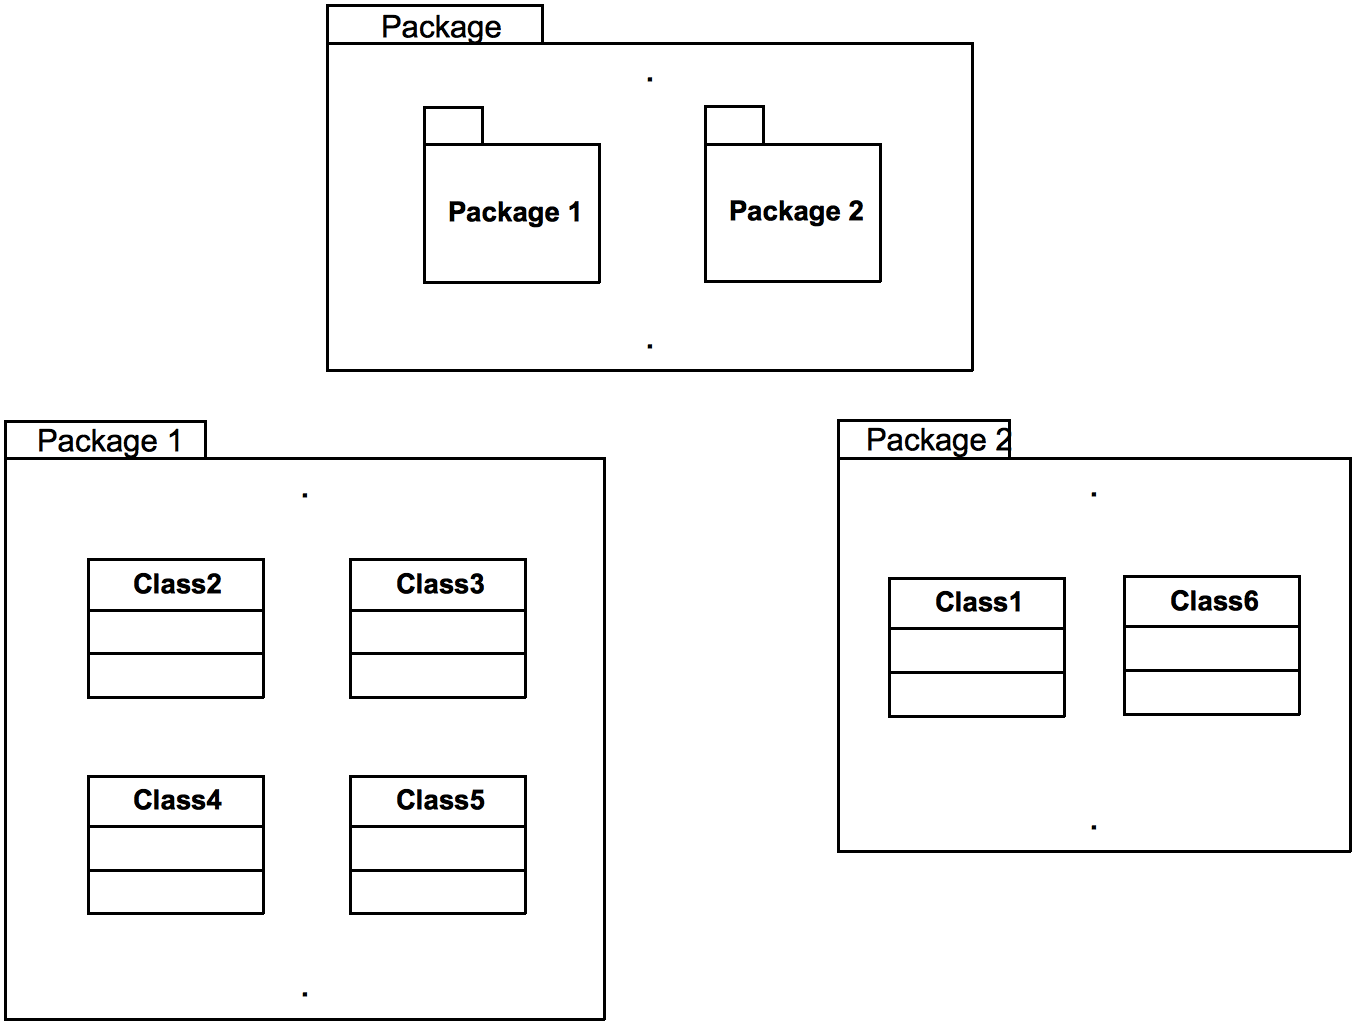
\includegraphics[scale=0.41]{ModeloDisenio/Fig2-1.png}
\end{siderules}
\newpage
\section{Realización de Casos de Uso}
Las realizaciones, están expresadas en términos de estructura e interacciones entre instancias que respeten dicha estructura. Concretamente, la parte estructural de una realización es un diagrama de clases conteniendo clases del modelo; la parte dinámica es un conjunto de diagramas de interacción que ilustran el flujo de mensajes entre instancias de las clases de la parte estructural correspondiente. 

\begin{siderules}
Esta sección está dividida por colaboración. Una colaboración es la realización de uno o más casos de uso. Para cada colaboración habrá una sección que muestre su diseño. El nombre de una colaboración corresponde al nombre del caso de uso que realiza, o el nombre del “área temática” determinada por el conjunto de casos de uso que realiza. La estructura para presentar la información será la siguiente:

\subsection{Colaboración 1}
En esta sección se presenta la colaboración que realiza uno o más casos de uso. Simplemente se realiza un diagrama como el de la figura 3-1, en el cual se indica el nombre de la colaboración y los casos de uso que realiza.

\begin{figure}[H]
\centering
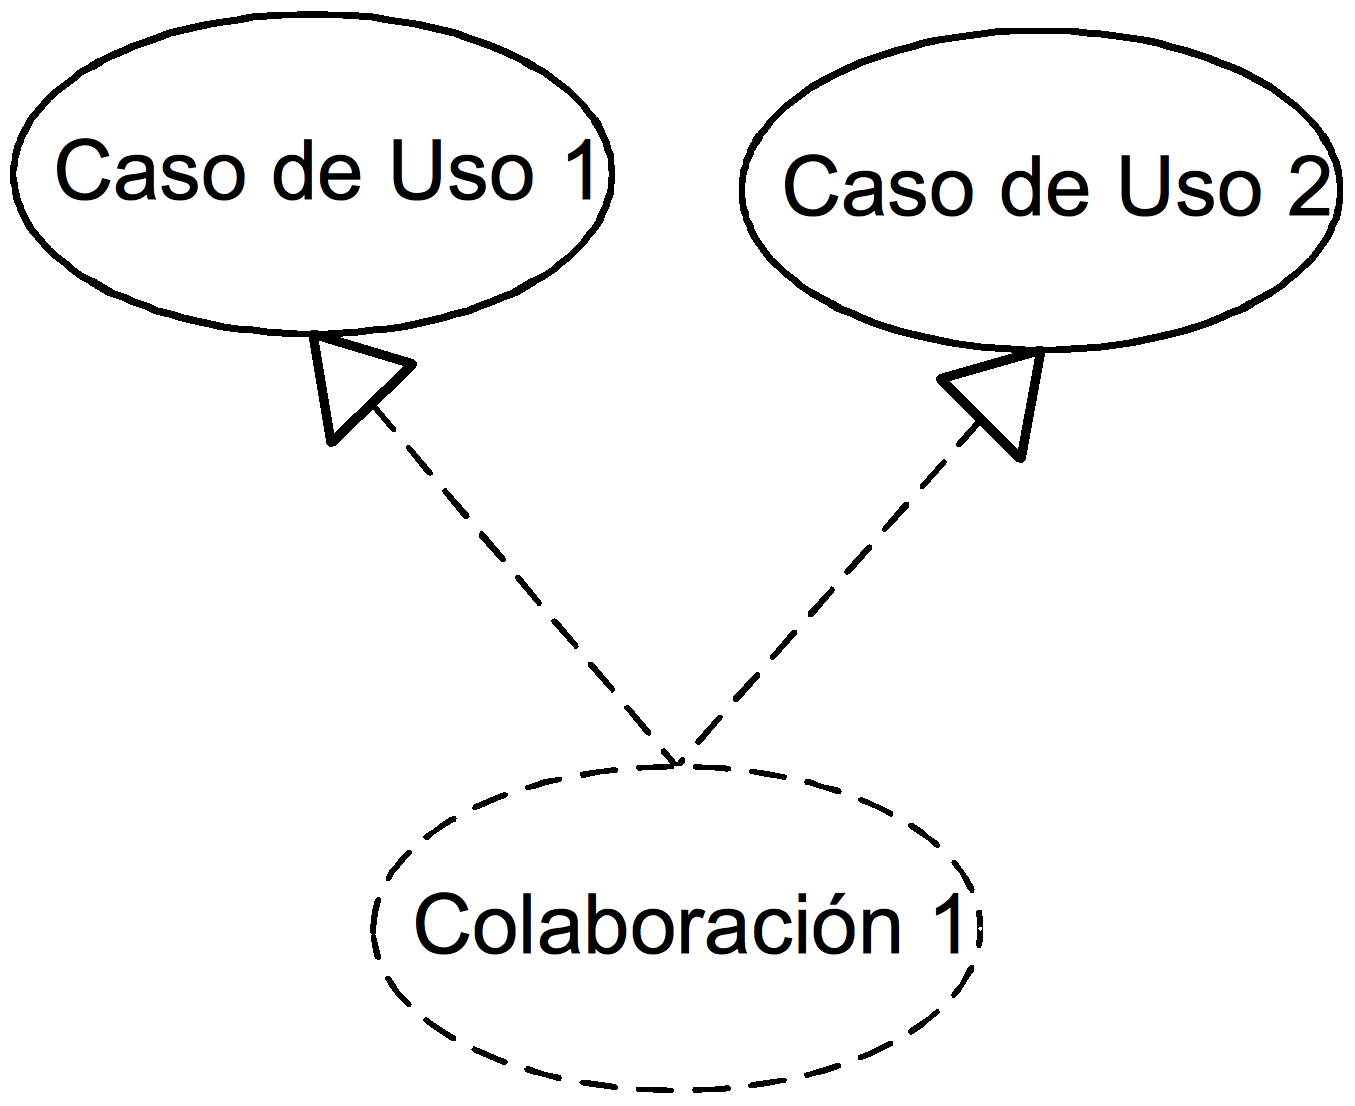
\includegraphics[scale=0.15]{ModeloDisenio/Fig3-1.png}
\caption{Colaboración}
\end{figure}
\subsubsection{Estructura}
En esta sección se presenta el diagrama de clases correspondiente al diseño de ésta colaboración.

Es común que el tamaño de este diagrama complique su presentación en una sola carilla. En este caso, es permisible separar el diagrama en varias hojas con distintos niveles de detalle. Por ejemplo se puede mostrar un diagrama que tenga sólo las clases y dependencias entre las mismas, y luego varios diagramas para mostrar cada clase en detalle pero sin sus relaciones con otras clases.

\begin{figure}[H]
\centering
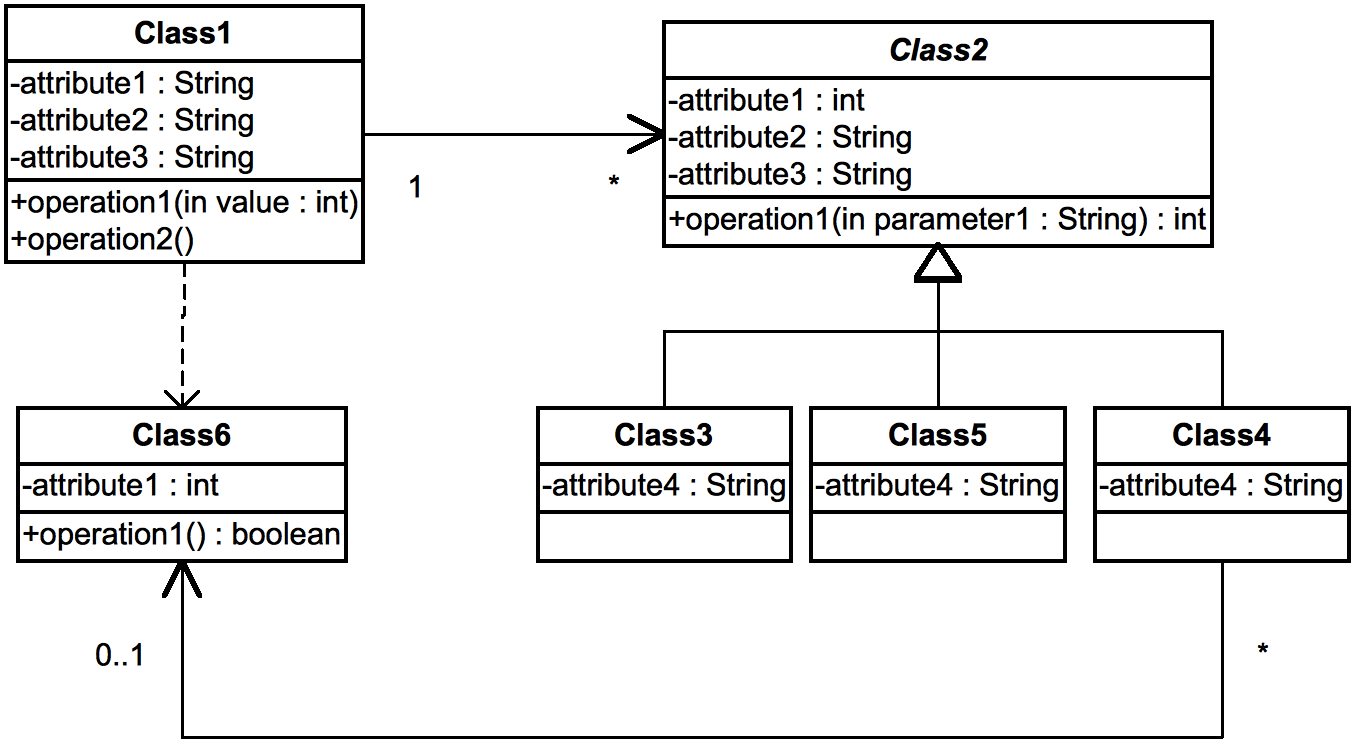
\includegraphics[scale=0.42]{ModeloDisenio/Fig3-2.png}
\caption{Diagrama de Clases de Diseño}
\end{figure}

\subsubsection{Interacciones}
En esta sección se presentan los diagramas de comunicación para representar los aspectos dinámicos de la colaboración. Por cada operación se agrega la siguiente información.

\subsubsubsection{Diagramas de comunicación de la operación 1}
En esta sección se presenta el diagrama de comunicación de la operación indicada y un detalle de la asignación de responsabilidades correspondientes al diagrama.

A modo de ejemplo se incluye lo siguiente:\\
\begin{figure}[H]
\centering
\includegraphics[scale=0.6]{ModeloDisenio/Fig3-3.png}
\captionsetup{justification=centering}
\caption{Diagrama de comunicación para la\\ operación Obtener el tamaño del sistema de archivos}
\end{figure}

Asignación de responsabilidades:
\begin{itemize}
\item Controller de la operación:  FileSystem.
\item Creador de Items:  FileSystem.
\item Destructor de Items:  Item.  FileSystem será responsable del Item raíz en el árbol del sistema de archivos.
\end{itemize}

\subsubsection{Design Patterns}
En esta sección se indican todos los Design Patterns involucrados en el diseño de la colaboración de esta sección. En caso de que la aplicación de este Design Pattern ya haya sido documentada (esto implica que las clases involucradas en el patrón sean las mismas) en alguna sección anterior sólo debe hacerse referencia a la misma. En caso que no se haya aplicado ningún Design Pattern esta sección no debe incluirse.

\subsubsubsection{Design Pattern 1}
Debe haber una sección como está por cada Design Pattern aplicado. Se debe indicar qué clases están involucradas, qué roles cumplen las mismas, y a su vez se debe dar una explicación textual que justifique su utilización.

A modo de ejemplo se incluye la siguiente especificación de un Design Pattern:
Dadas estas características se diseñó el sistema de archivos aplicando el Design Pattern Composite. 

Las clases involucradas son:
\begin{itemize}
\item[--] Item, que cumple el rol de Component.
\item[--] Archivo, que cumple el rol de Leaf.
\item[--] Directorio, que cumple el rol de Composite.
\end{itemize}
\end{siderules}

\section{Criterios Generales}
\begin{siderules}
En el diseño de un sistema típicamente existen ciertas decisiones que no se toman de manera local al realizar el diseño de un caso de uso sino que responden a una consideración global de las distintas funcionalidades que el sistema debe ofrecer.

A su vez suelen existir ciertos problemas que aparecen repetidamente en el sistema, y que por mantener una coherencia interna y facilitar la comprensión del diseño se resuelven siempre de la misma forma.

Esta sección está dedicada a explicar estos dos tipos de cuestiones que son globales y no dependen de cada caso de uso particular sino de una concepción general del diseño del sistema. Obviamente en caso de no existir ninguna decisión de este tipo, esta sección puede ser descartada.

A continuación se muestra un ejemplo:

En primer lugar, para asignar la responsabilidad de atender las operaciones del sistema se decidió definir un controlador para las operaciones relacionadas con dar de alta, baja y requerir información sobre los clientes; otro para este tipo de operaciones sobre los descuentos; y otro para este tipo de operaciones sobre las ventas.

También se definió un controlador que se encarga de las autorizaciones, ya sea para autenticar un local a la hora de inicializar el sistema, o para autorizar las tarjetas cuando se desea efectuar una compra o también para saber cuántos puntos genera una venta con un determinado monto. También se definió otro controlador para poder trabajar con el local que se encuentra logueado, es decir, en sesión. Todos estos controladores son Singleton.

En general se tomó el criterio de asignar la responsabilidad de destrucción de una instancia al mismo objeto que posee la responsabilidad de crearla.
\end{siderules}
\end{document}